\section{Rudin Chapter 14}

The \textbf{direction} of $z$ is $A[z]\coloneqq\frac{z}{\lvert z \rvert}$.

\begin{definition}[preserves angles]
\begin{figure}[H]
\centering
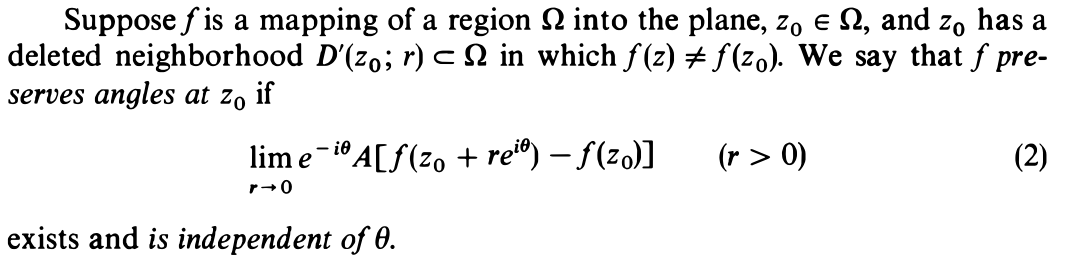
\includegraphics[width=\textwidth]{rudin-conformal-mapping-2025052220.png}
% \caption{}
\label{}
\end{figure}
\end{definition}
In less precise language, the requirement is that for any two rays $L$ and $L'$, starting at $z_0$, the angle which their images $f(L)$ and $f(L')$ make at $f(z_0)$ is the same as that made by $L$ and $L'$, in size as well as in orientation.

The property of preserving angles at each point of a region is characteristic of holomorphic functions whose derivative has no zero in that region.

\begin{definition}
Suppose $\mathscr{F} \subset H(\Omega)$, for some region $\Omega$. We call $\mathscr{F}$ a \textbf{normal family} if every sequence of members of $\mathscr{F}$ contains a subsequence which converges\footnote{may converges to $\infty$} uniformly on compact subsets of $\Omega$. The limit function is not required to belong to $\mathscr{F}$.
\end{definition}
\begin{theorem}
Suppose $\mathscr{F} \subset H(\Omega)$ and $\mathscr{F}$ is uniformly bounded on each compact subset of the region $\Omega$. Then $\mathscr{F}$ is a normal family.
\end{theorem}
\subsection{The Riemann Mapping Theorem}

\begin{figure}[H]
\centering
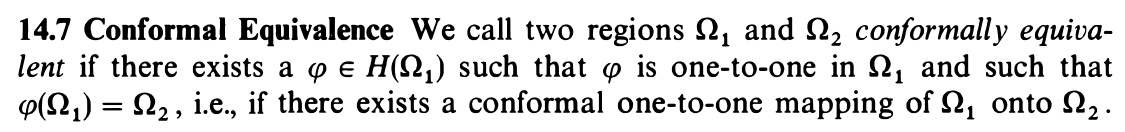
\includegraphics[width=\textwidth]{1-rudin-conformal-mapping-2025052220.png}
% \caption{}
\label{}
\end{figure}

The Riemann mapping theorem reduces the study of $H(\Omega)$ to $H(U)$, for any simply connected proper subregion of the plane.

\begin{figure}[H]
\centering
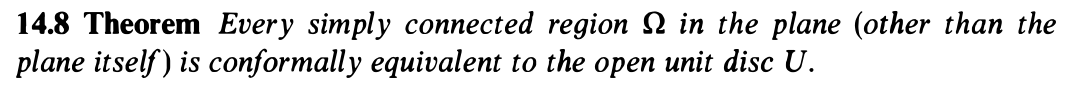
\includegraphics[width=\textwidth]{2-rudin-conformal-mapping-2025052220.png}
% \caption{}
\label{}
\end{figure}

\subsection{The class \texorpdfstring{$\mathscr{S}$}{mathscrS}}

\begin{definition}
$\mathscr{S}$ is the class of all $f \in H(U)$ which are injective in $U$ and which satisfy
\[
\begin{gathered}
f(0)=0, \quad f^{\prime}(0)=1 .
\end{gathered}
\]Thus every $f \in \mathscr{G}$ has a power series expansion
\[
f(z)=z+\sum_{n=2}^{\infty} a_n z^n \quad(z \in U) .
\]
\end{definition}
The class $\mathscr{S}$ is not closed under addition or multiplication, but has many other interesting properties. We shall develop only a few of these in this section. Theorem 14.15 will be used in the proof of Mergelyan's theorem, in Chap. 20.

\begin{figure}[H]
\centering
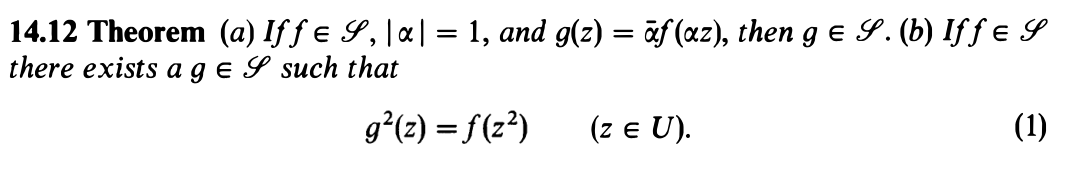
\includegraphics[width=\textwidth]{rudin-conformal-mapping-2025052221.png}
% \caption{}
\label{}
\end{figure}

\begin{proof}
(a) is clear. To prove (b), write $f(z)=z\varphi(z)$. Then $\varphi\in H(U),\varphi(0)=1$, and $\varphi$ has no zero in $U$ since $f$ has no zero in $U\setminus \{ 0 \}$. Hence there exists $h\in H(U)$, with $h(0)=1$, $h^2(z)=\varphi(z)$. Put
\[
g(z)=zh(z^2)\qquad z\in U
\]
Then $g^2(z)=z^2h^2(z^2)=z^2\varphi(z^2)=f(z^2)$. NTS: $g\in \mathscr{S}$. Clearly, $g(0)=0$, $g'(0)=1$. For $z, w\in U$, $g(z)=g(w)$, then, $z^2=w^2$; as $f$ is injective, $z=\pm w$. If $z=-w$, then $g(z)=zh(z^2)=-wh(w^2)=-g(w)$; it follows that $g(z)=g(w)=0$, and since $g$ has no zero in $U\setminus \{ 0 \}$, we have $z=w=0$.
\end{proof}

\begin{theorem}[area theorem (Theorem 14.13)]
If $F \in H(U-\{0\})$, $F$ is one-to-one in $U$, and
\[
F(z)=\frac{1}{z}+\sum_{n=0}^{\infty} \alpha_n z^n \quad(z \in U),
\]then
\begin{equation}
\sum_{n=1}^{\infty} n\left|\alpha_n\right|^2 \leq 1 .
\label{1a9dd9}
\end{equation}
\end{theorem}

\begin{proof}
WLOG, assume $\alpha_0=0$, $\alpha_1$ is real. Put $U_{r}\coloneqq \{ \lvert z \rvert<r \}$, $C_{r}\coloneqq \{ \lvert z \rvert=r \}$, $V_{r}\coloneqq \{ r<\lvert z \rvert<1 \}$. Then $F(U_{r})$ is a neighborhood of $\infty$; the sets $F(U_{r})$, $F(C_{r})$ and $F(V_{r})$ are disjoint, as $f$ is injective. $F(V_{r})$ is in the interior of $F(C_{r})$. Write
\[
F(z)=\frac{1}{z}+\alpha_1z+\varphi(z)\qquad z\in U
\]
$F=u+i v$ and
\[
A=\frac{1}{r}+\alpha_1r\qquad B=\frac{1}{r}-\alpha_1r
\]
For $z=re^{ i\theta }$, we then obtain
\[
u=A\cos\theta+\mathrm{Re}\varphi \qquad \text{and}\qquad v=-B\sin\theta+\mathrm{Im}\varphi
\]
Then
\[
\frac{u^2}{A^2}+\frac{v^2}{B^2}=1+\underbrace{ \frac{2\cos\theta}{A} }_{ =O(r) }\underbrace{ \mathrm{Re}\varphi }_{ =O(r^2) }+\underbrace{ \left( \frac{\mathrm{Re}\varphi}{A} \right)^2 }_{ =O(r^{6}) }-\underbrace{ \frac{2\sin\theta}{B}\mathrm{Im}\varphi }_{ =O(r^{3}) }+\underbrace{ \left( \frac{\mathrm{Im}\varphi}{B} \right)^2 }_{ =O(r^{6}) }
\]
There exists $\eta>0$, if sufficiently small $r$, we have
\[
\frac{u^2}{A^2}+\frac{v^2}{B^2}<1+\eta r^3\qquad z=re^{ i\theta }
\]
This says $F(C_{r})$ lies in the interior of ellipse $E_{r}$, whose semiaxes are $A\sqrt{ 1+\eta r^{3} }$ and $B\sqrt{ 1+\eta r^{3} }$, and which therefore bounds an area
\begin{equation}
\pi AB(1+\eta r^{3})=\pi\left( \frac{1}{r}+\alpha_1r \right)\left( \frac{1}{r}-\alpha_1r \right)(1+\eta r^3)\leq \frac{\pi}{r^2}(1+\eta r^{3})
\label{4fdc67}
\end{equation}

Since $F(V_{r})$ is in the interior of $F(C_{r})$, the area of $F(V_{r})$ is no larger than \cref{4fdc67}. The Cauchy-Riemann equations show that the Jacobian of $(x,y)\to(u,v)$ is $\lvert F' \rvert ^2$, then
\[
\begin{aligned}
\frac{\pi}{r^2}(1+\eta r^2) & \geq \iint_{V_{r}}\lvert F' \rvert ^2 \\
 & =\int_{r}^{1} t \, \mathrm{d}t\int_{0}^{2\pi} \left\lvert  -t^{-2}e^{ -2i\theta }+\sum_{n=1}^{\infty} n\alpha _nt^{n-1}e^{ i(n-1)\theta }  \right\rvert  \, \mathrm{d}\theta  \\
 & =2\pi \int_{r}^{1} \left( t^{-3}+\sum_{n=1}^{\infty} n^2\lvert \alpha _n \rvert ^2t^{2n-1} \right) \, \mathrm{d}t \\
  & =\pi\left[ r^{-2}-1+\sum_{n=1}^{\infty} n \lvert \alpha _n \rvert ^2(1-r^{2n}) \right]
\end{aligned}
\]
Thus
\[
\sum_{n=1}^{N} n \lvert \alpha _n \rvert ^2(1-r^{2n})\leq 1+\eta r\qquad \forall N>0
\]
Let $r\to0$, then let $N\to \infty$. We are done!
\end{proof}

\begin{corollary}
Under the same hypothesis in \cref{1a9dd9}, $\lvert \alpha_1 \rvert\leq1$.\label{74fd16}
\end{corollary}

\begin{figure}[H]
\centering
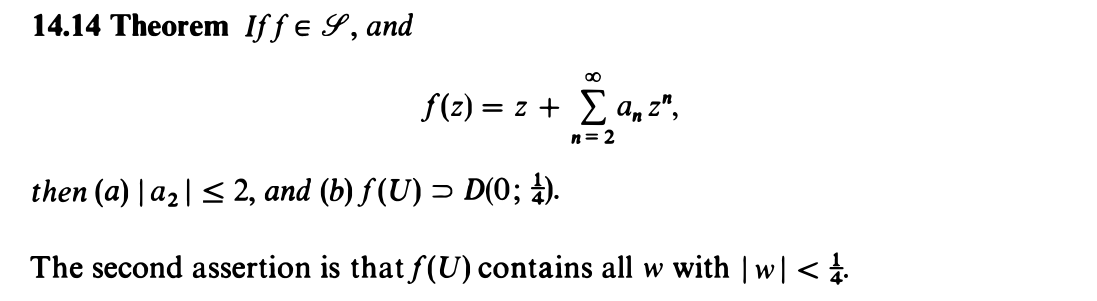
\includegraphics[width=\textwidth]{rudin-conformal-mapping-2025052222.png}
% \caption{}
\label{}
\end{figure}

\begin{note}
The second assertion is that $f(U)$ contains all $w$ with $\lvert w \rvert<\frac{1}{4}$.
\end{note}
\begin{proof}
(a) By theorem 14.12, there exists $f\in \mathscr{S}$ s.t. $g^2(z)=f(z^2)$. Denote $G\coloneqq1/g$, then \cref{1a9dd9} applies to $G$ and this yields (a). Since
\[
f(z^2)=z^2+\sum_{n=2}^{\infty} a_nz^{2n}
\]
we have
\[
g(z)=z\left( 1+\frac{1}{2}a_2z^2+\dots \right)
\]
and hence
\[
G(z)=\frac{1}{z}\left( 1-\frac{1}{2}a_2z^2+\dots \right)
\]
By \cref{74fd16}, $\lvert a_2 \rvert\leq2$.

To prove (b), suppose $w\not\in f (U)$. Define
\[
h(z)=\frac{f(z)}{1-f(z)/w}
\]
Then $h\in H(U)$, $h$ is injective in $U$, and
\[
h(z)=(z+a_2z^2+\dots)\left( 1+\frac{z}{w} +\dots\right)=z+\left( a_2+\frac{1}{w} \right)z^2+\dots
\]
so that $h\in \mathscr{S}$. Apply (a) to $h$: we have $\left\lvert  a_2+\frac{1}{w}  \right\rvert<2$ and since $\lvert a_2 \rvert\leq2$, we finally obtain $\lvert 1/w  \rvert\leq4$. So $\lvert w \rvert\geq\frac{1}{4}$ for every $w\not\in f (U)$. This complete the proof.
\end{proof}

Moreover, given any $\alpha\neq0$, one can find entire $f$ with $f(0)=0$, $f'(0)=1$, that omit the value $\alpha$. For example,
\[
f(z)=\alpha(1-e^{ -z/\alpha })
\]
Of course, by Theorem 14.14, that $f$ is injective in $U$ and $\lvert \alpha \rvert<\frac{1}{4}$ cannot happen at the same time.

\begin{figure}[H]
\centering
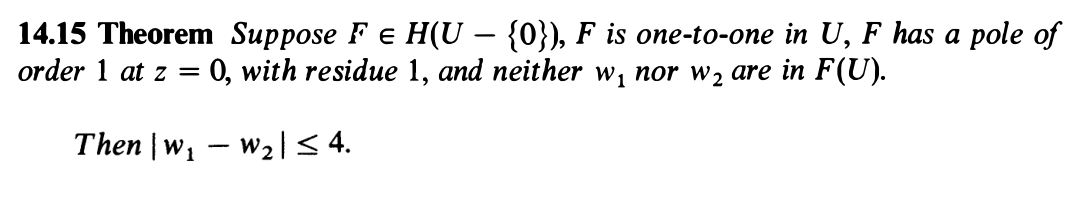
\includegraphics[width=\textwidth]{1-rudin-conformal-mapping-2025052222.png}
% \caption{}
\label{}
\end{figure}

\begin{proof}
Let $f\coloneqq 1/(F-w_1)$, then $f\in \mathscr{S}$, hence $f(U)\supset B_{\frac{1}{4}}(0)$, so the image of $U$ under $F-w_1$ contains all $w$ with $\lvert w \rvert>4$. Since $w_2-w_1$ is not in this image, we have $\lvert w_2-w_1 \rvert\leq4$.
\end{proof}
